\documentclass[a4paper, 11pt, oneside]{article}
\usepackage[UTF8]{ctex}
\usepackage{geometry}
\usepackage{amsmath}
\usepackage{amsthm}
\usepackage{graphicx}
\usepackage{hyperref}

\setcounter{secnumdepth}{6}
\geometry{left = 2.5cm, right = 2.5cm, top = 2.5cm, bottom = 2.5cm}

\newcommand{\bol}[1]{\textbf{#1}}
\newcommand{\mbol}[1]{\boldsymbol{#1}}
\newcommand{\hahacite}[1]{\textsuperscript{\textsuperscript{\textsuperscript{\cite{#1}}}}}
\newcommand{\diff}{\mathrm{d}}
\newcommand{\ccite}[1]{\cite{#1}}

\title{物理总结}
\author{Xiaoyu Xue \\ xiaoyu.xue@acm.org}
\date{\today}

\begin{document}
\maketitle
\newpage
\tableofcontents
\newpage

\section{前置知识}
\subsection{数学}
\subsubsection{向量}
所有有方向的变量称为向量,一般有两种写法上方加箭头,或者粗体,本文中所有的向量都用粗体表示,比如
\begin{displaymath}
	\bol{a} \Longleftrightarrow \overrightarrow{a}
\end{displaymath}
\paragraph{向量的维度}\quad\\
\indent 二维向量$\bol{a} = (x,y)$,三维向量$\bol{a}=(x,y,z)$\\
\paragraph{向量的长度}\quad\\
\begin{displaymath}
	\vert\bol{a}\vert = \sqrt{x^2 + y^2 + z^2}
\end{displaymath}
\paragraph{向量加减法以及平行四边形法则}\quad\\
\indent$\bol{a} = (x_1, y_1, z_1)$,$\bol{b} = (x_2, y_2, z_2)$
\begin{displaymath}
	\bol{a} + \bol{b} = (x_1 + x_2, y_1 + y_2, z_1 + z_2)
\end{displaymath}
\begin{figure}[!h]
\center
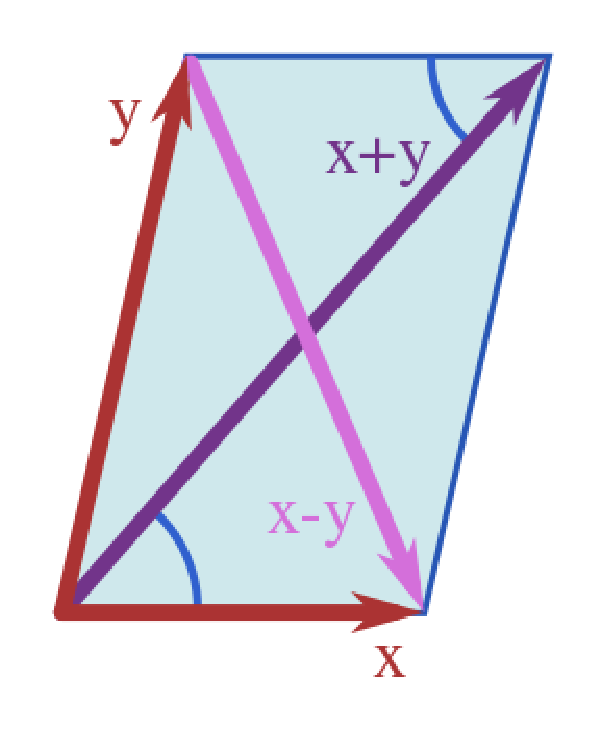
\includegraphics[scale=0.5]{./asset/parallelogram_law.eps}
\caption{平行四边形法则}
\end{figure}
\paragraph{向量数乘}\quad\\
\indent 向量点乘的结果是一个标量(数值)
\begin{displaymath}
	c\bol{a} = (cx, cy, cz)
\end{displaymath}
\paragraph{向量点乘}\quad\\
\indent 向量的点乘结果是一个标量(数值)
\begin{displaymath}
	\vert\bol{a}\cdot\bol{b}\vert = \vert \bol{a} \vert \vert \bol{b} \vert \cos{\theta} = x_1y_1 + x_2y_2
\end{displaymath}
\paragraph{向量叉乘}\quad\\
\indent 向量叉乘的结果是一个向量,长度为
\begin{displaymath}
	\vert \bol{a} \times \bol{b} \vert = \vert\bol{a}\vert \vert\bol{b}\vert \sin{\theta}
\end{displaymath}
方向为:请注意是左手系还是右手系
\begin{figure}[!h]
\center
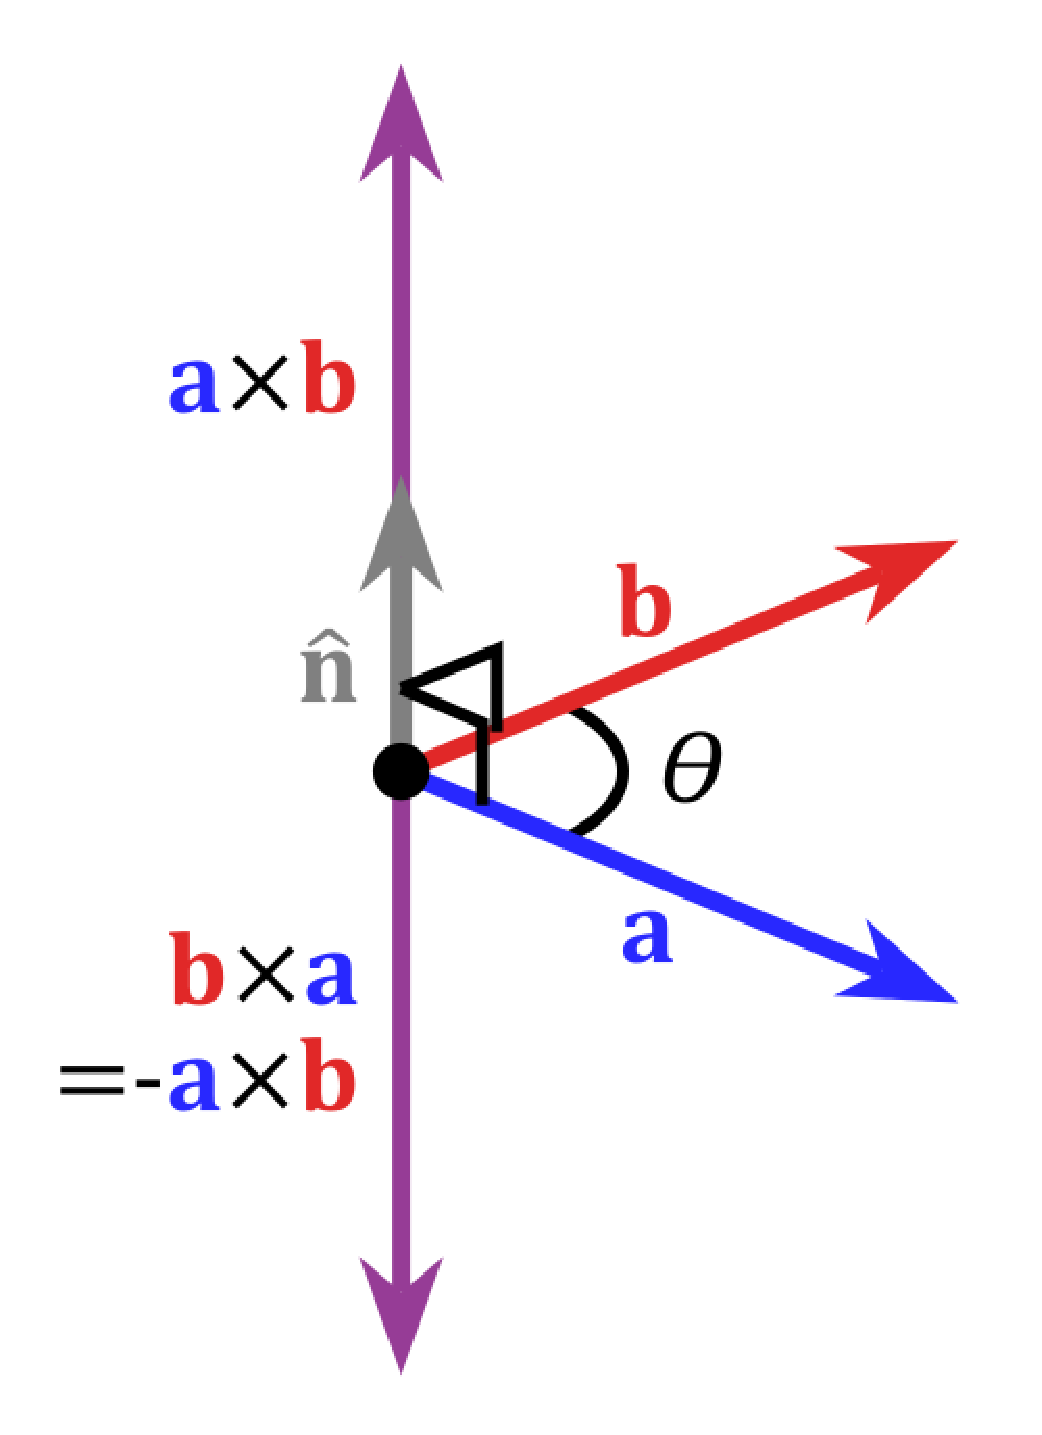
\includegraphics[scale=0.3]{./asset/vector_times.eps}
\caption{向量叉乘的方向}
\end{figure}
\subsubsection{初等函数}
\begin{itemize}
	\item 线性函数/一次函数(单变量)$y = f(x) = ax+b$
	\item 二次函数 (单变量)$y = f(x) = ax^2 + bx + c$
\end{itemize}
确保会求它们的最值
\newpage
\section{运动学}
\subsection{位移}
定义:由初位置到末位置的一段有向线段(向量),单位: $m$\\
假设点A的位置为$\bol{a} = (x_1, y_1, z_1)$,点B的位置为$\bol{b} = (x_2, y_2, z_2)$,A到B的位移为$\bol{x} = \bol{b} - \bol{a} = (x_2 - x_1 , y_2 - y_1, z_2 - z_1)$

\subsection{速度}
定义:一个物体的速度定义成在某个参考系下它的位置的变换率,是一个随时间变化的函数,可以用$\bol{v}(t)$表示,单位: $m/s$
\subsubsection{平均速度}
\begin{displaymath}
	\bar{\bol{v}} = \frac{\Delta \bol{x}}{\Delta t}
\end{displaymath}
其中$\Delta \bol{x}$表示位移,$\Delta t$表示经历的时间
\subsubsection{瞬时速度}
当经历的时间$\Delta t$无限接近于0时,就得到了瞬时速度
\begin{displaymath}
	\bol{v} = \lim_{\Delta t \to 0}\frac{\Delta \bol{x}}{\Delta t} = \frac{\diff\bol{x}}{\diff t}
\end{displaymath}
\subsubsection{匀速直线运动}
匀速直线运动就是指方向和大小都不改变的速度
\newpage
\section{力学(静力学)}
\subsection{力}
在物理学中,力是任何导致自由物体历经速度、方向或外型的变化的影响。\\
你们所谓的三要素:
\begin{enumerate}
	\item 大小
	\item 方向
	\item 作用点
\end{enumerate}
从第2点就可以知道力就是一个向量,力的字母表示通常是$\bol{F}$,经典力学通常涉及到牛顿运动定律,我们讨论的也都是经典力学的范围。力的单位为: 牛顿(N)
\subsection{力的种类}
\subsubsection{基础力}
\paragraph{重力}\quad\\
\indent 现在所称的重力,直到艾萨克·牛顿的工作之前,都没有被认定是万有的。这个朝向地球表面的由重力产生的加速度通常以 $\bol{g}$表示,有一个大约是9.81米每平方秒的大小(这个是从海平面测量且跟位置有关)且指向地心。 这个观测意味着地球表面上作用在物体上的重力直接地与物体质量成正比。因此一个有质量为$m$的物体所受的重力为
\begin{displaymath}
	\bol{G} = m\bol{g}
\end{displaymath}
此外呢$\bol{g}$的另外一个单位就是$N/kg$,\underline{方向永远竖直向下}
\paragraph{*电磁力}
\paragraph{*核力}
\subsubsection{非基础力}
\paragraph{支持力与弹力}\quad\\
在物理学中,支持力是由于支撑面发生形变,对被支持的物体产生的弹力,通常称为支持力。支持力可以用符号“N”来表示。
\paragraph{*张力}
\paragraph{浮力}\quad\\
$F_{\text{浮}} = \rho g V$ = $\rho g h S$ = $\Delta F_{\text{压}}$
\paragraph{摩擦力}
\subparagraph{滑动摩擦力}
\subparagraph{滚动摩擦力}
\subparagraph{静摩擦力}\quad\\
\indent 如何判断静摩擦力的方向:与相对运动趋势相反
\paragraph{TMD假象力}
\subsection{牛顿运动定律}
\begin{itemize}
	\item 牛顿第一定律$\underline{\quad\quad\quad\quad\quad\quad\quad\quad\quad\quad\quad\quad\quad\quad\quad\quad\quad\quad}$
	\item *牛顿第二定律
	\item 牛顿第三定律$\underline{\quad\quad\quad\quad\quad\quad\quad\quad\quad\quad\quad\quad\quad\quad\quad\quad\quad\quad}$
\end{itemize}
\subsection{受力分析}
\subsubsection{全部分析对!!!}
分别对A,B以及地面做受力分析\;!!!!!!!!!!!!!!!!!!!!!!!!!!!!!!!!!!!!!!!!!!!!!!!!!!!!!!!!!!!!!!!!!!!!!!!!!!!!!!!!!! \\
\begin{figure}[!h]
\center
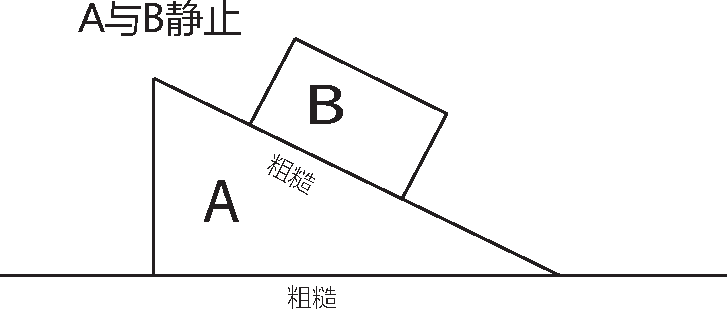
\includegraphics[scale=0.8]{./asset/force_analysis_1.pdf}
\caption{习题1}
\end{figure}
\begin{figure}[!h]
\center
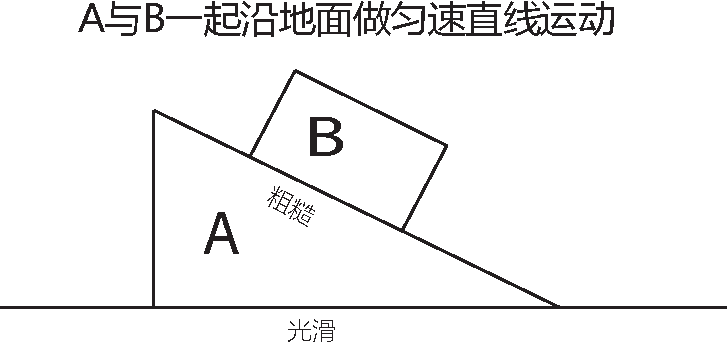
\includegraphics[scale=0.8]{./asset/force_analysis_2.pdf}
\caption{习题2}
\end{figure}
\begin{figure}[!h]
\center
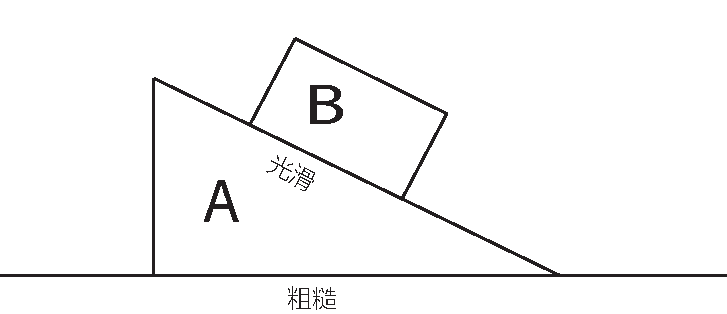
\includegraphics[scale=0.8]{./asset/force_analysis_3.pdf}
\caption{习题3}
\end{figure}
\begin{figure}[!h]
\center
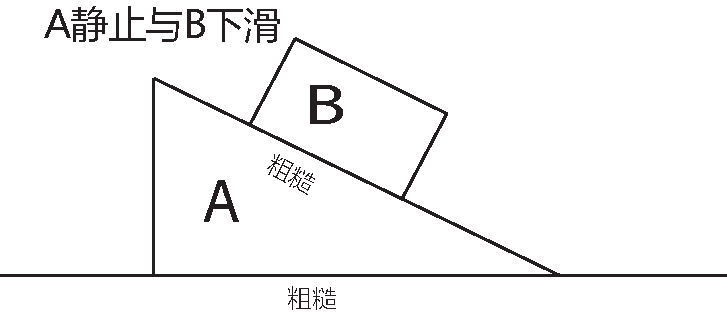
\includegraphics[scale=0.8]{./asset/force_analysis_4.pdf}
\caption{习题4}
\end{figure}
\begin{figure}[!h]
\center
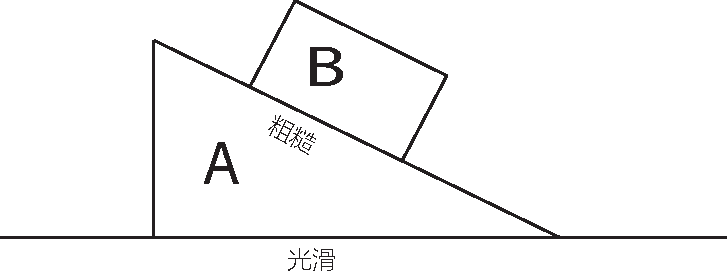
\includegraphics[scale=0.8]{./asset/force_analysis_5.pdf}
\caption{习题5}
\end{figure}
\begin{figure}[!h]
\center
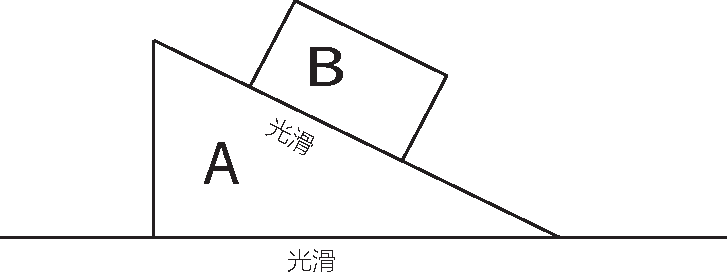
\includegraphics[scale=0.8]{./asset/force_analysis_6.pdf}
\caption{习题6}
\end{figure}
\subsubsection{你所谓的最怕的浮力}
分析每个图中等冰块融化后,水面会不会溢出\\
\begin{figure}[!h]
\center
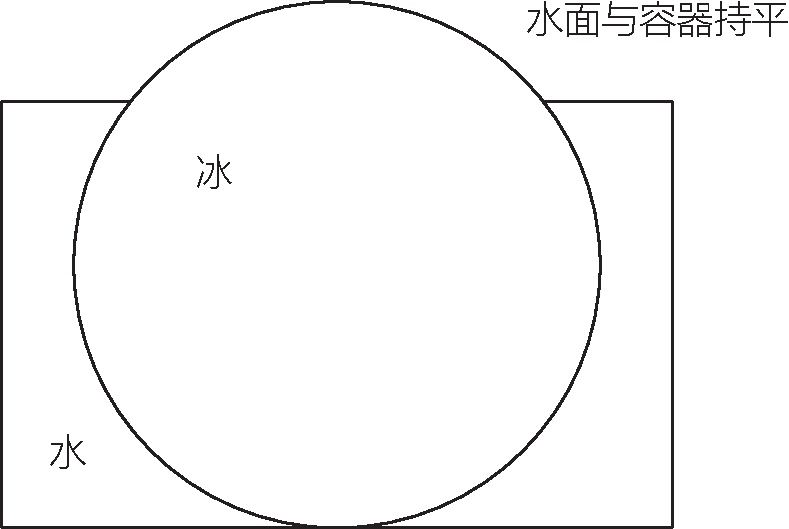
\includegraphics[scale=0.6]{./asset/buoyancy_1.pdf}
\caption{习题7}
\end{figure}
\\ \quad \\
\begin{figure}[!h]
\center
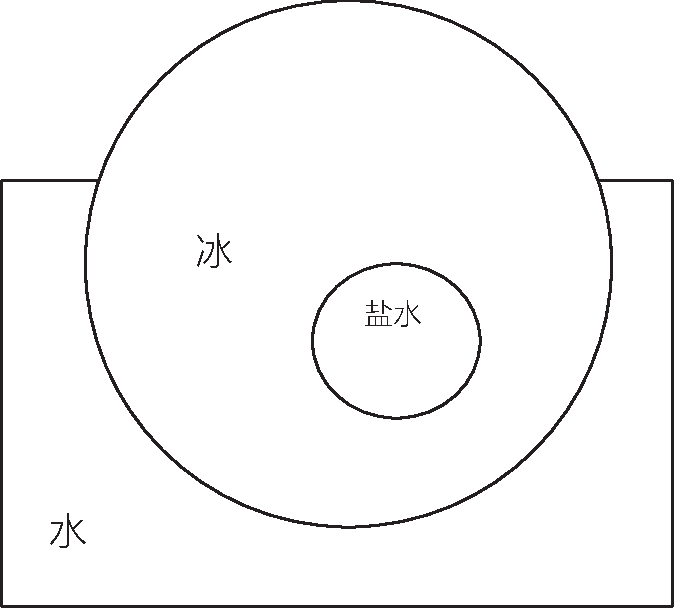
\includegraphics[scale=0.6]{./asset/buoyancy_2.pdf}
\caption{习题8}
\end{figure}
\\
\begin{figure}[!h]
\center
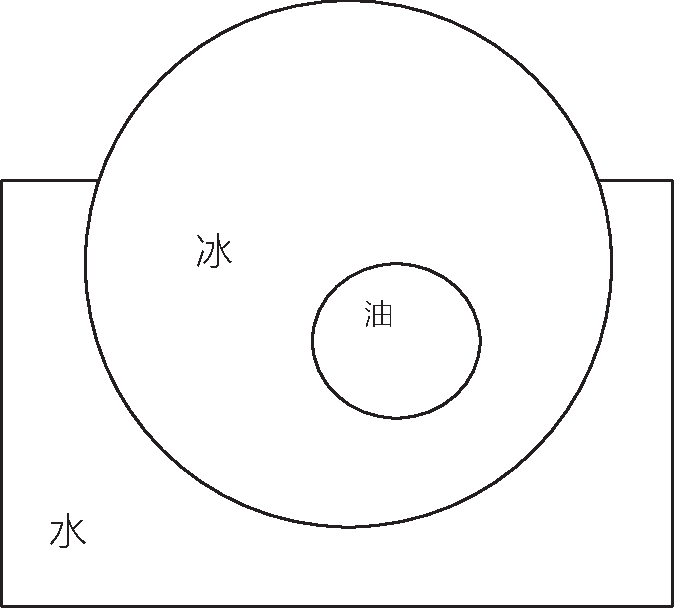
\includegraphics[scale=0.6]{./asset/buoyancy_3.pdf}
\caption{习题9}
\end{figure}
\end{document}